\documentclass[12pt]{article}
\usepackage[french]{babel}
\usepackage[utf8]{inputenc} % Required for inputting international characters
\usepackage[T1]{fontenc} % Output font encoding for international characters
\usepackage{textcomp}
\usepackage{graphicx}
\usepackage{mathpazo} % Palatino font
\usepackage{amsmath}
\usepackage{listings}
\usepackage{subcaption}
\usepackage{xcolor}
\usepackage{lscape}
\usepackage[onehalfspacing]{setspace}

\usepackage{geometry}
 \geometry{
 a4paper,
 left=35mm,
 right=35mm,
 top=40mm,
 bottom=40mm,
 }

\begin{document}
\begin{titlepage} % Suppresses displaying the page number on the title page and the subsequent page counts as page 1
	\newcommand{\HRule}{\rule{\linewidth}{0.5mm}} % Defines a new command for horizontal lines, change thickness here
	
	\center % Centre everything on the page
	
	%------------------------------------------------
	%	Headings
	%------------------------------------------------
	
	\textsc{\LARGE Ecole Centrale de Lille}\\[1cm] % Main heading such as the name of your university/college
	
	
    \begin{figure}[h!]
        \centering
        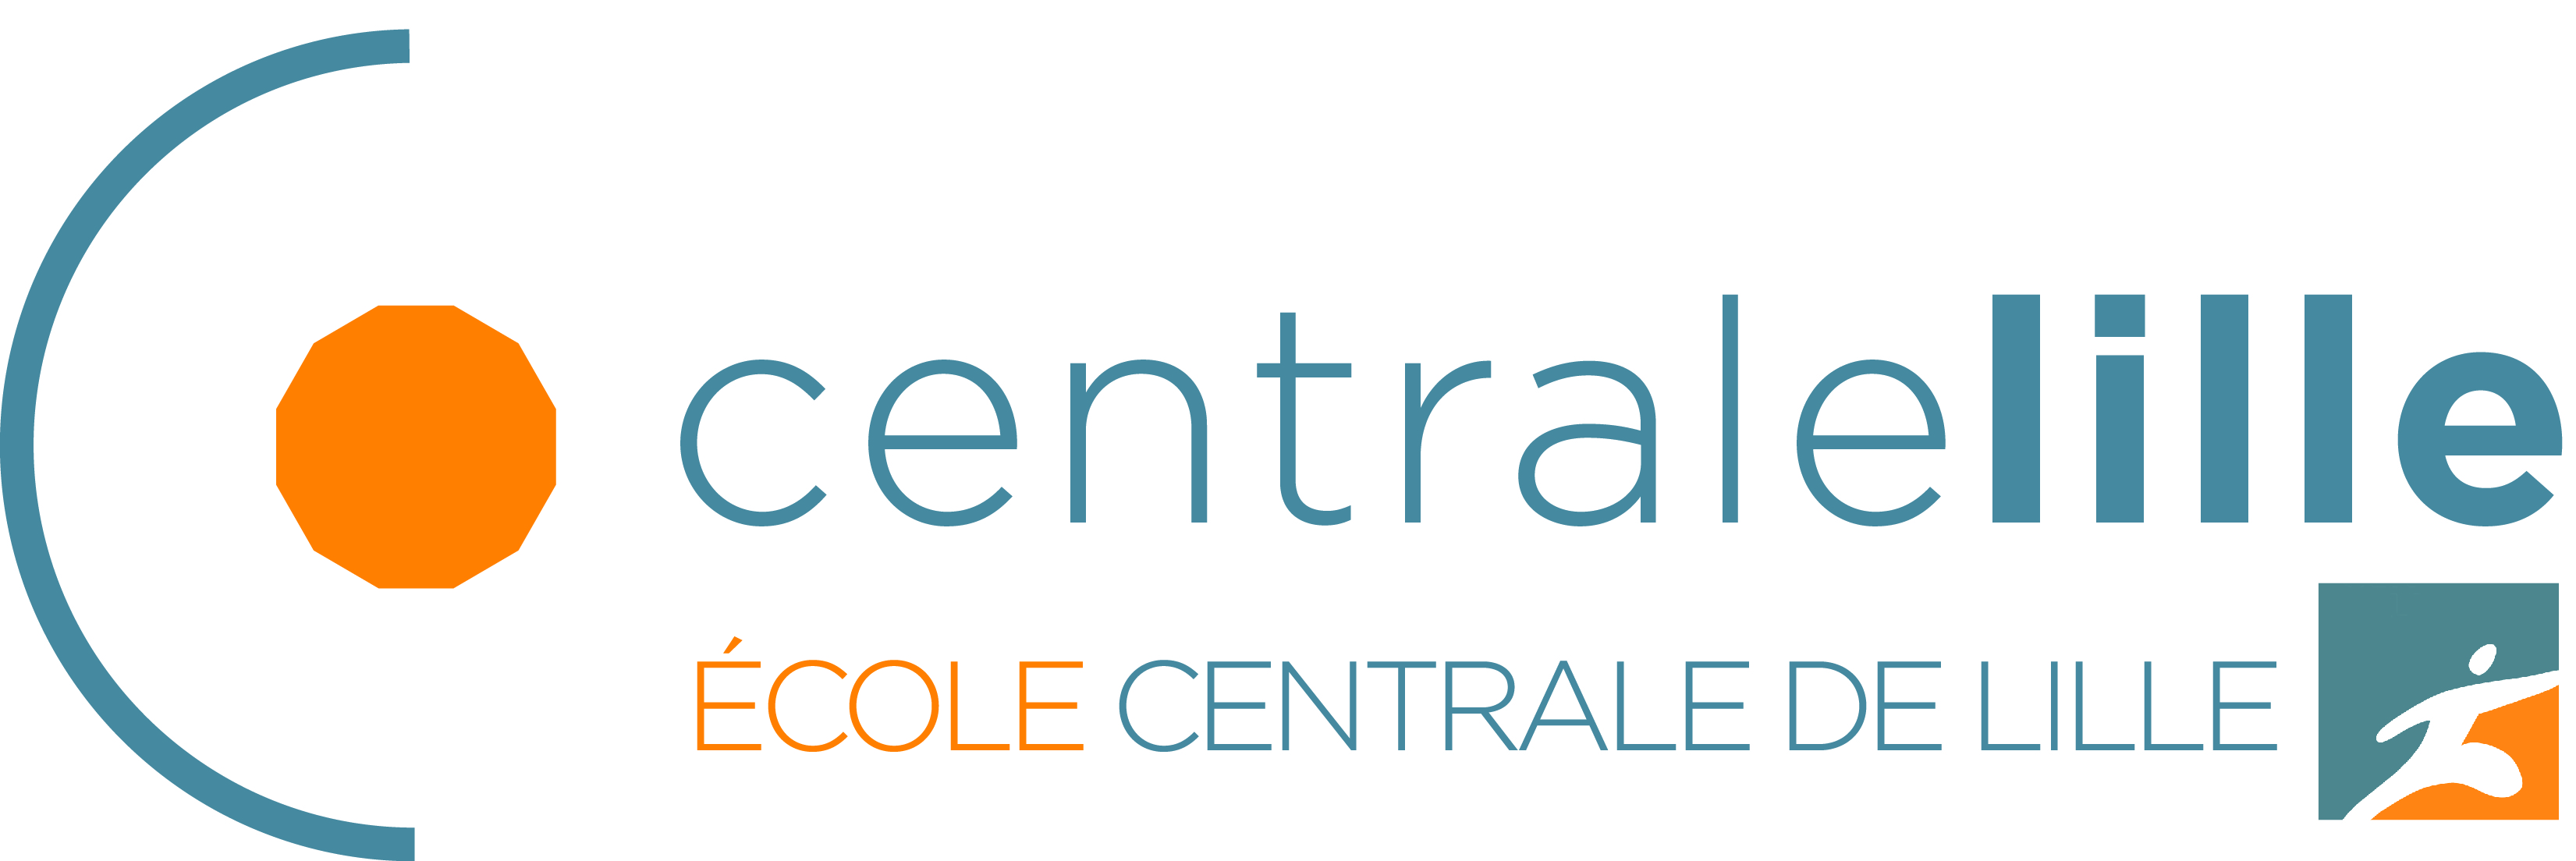
\includegraphics[width=0.6\textwidth]{logo_centrale.png}
        \label{LogoCentrale}
    \end{figure}
    
    \vfill
	
	%------------------------------------------------
	%	Title
	%------------------------------------------------
	
	\HRule\\[0.4cm]
	
	{\huge\bfseries Note de problématique: CIFRE vs non-CIFRE}\\[0.4cm] % Title of your document
	
	\HRule\\[1.0cm]
	
	%------------------------------------------------
	%	Author(s)
	%------------------------------------------------

	\begin{minipage}{0.4\textwidth}
		\begin{flushleft}
			\large
			\textit{Auteurs}\\
			E. \textsc{Le Guillou} \\
			I. \textsc{Thomas}\\
			A. \textsc{Rahier}\\
			M. \textsc{Lanvin}\\
			C. \textsc{Vo}
		\end{flushleft}
	\end{minipage}
	~
	\begin{minipage}{0.4\textwidth}
		\begin{flushright}
			\large
			\textit{Professeurs}\\
			J. P. \textsc{Richard}\\ % Supervisor's name
			C. \textsc{Belart} \\
			C. \textsc{Davy}
		\end{flushright}
	\end{minipage}

	\vfill
	
	\begin{center}
        %Nombre de mots : ?
    \end{center}
	%------------------------------------------------
	%	Date
	%------------------------------------------------
	
	\vfill\vfill % Position the date 3/4 down the remaining page
	
	{\large\today} % Date, change the \today to a set date if you want to be precise

	
	
	\vfill % Push the date up 1/4 of the remaining page
	
\end{titlepage}

\paragraph{Question initiale} % Que garder ?

Notre premier questionnement portait sur ce qu'était une thèse CIFRE. Nos questions cherchaient à nous faire découvrir ce qui se cachait derrière le terme de CIFRE.

Par exemple, quelles conditions de travail rencontre un doctorant CIFRE ? Ou bien à qui va la reconnaissance du travail effectué ? Les débouchés après la thèse sont-ils meilleurs ?

Ces simples questions nous ont ensuite mené à formuler un questionnement plus large qui pourrait mener lieu à un travail épistème.

% utile ? vaut-il mieux parler des axes de réflexions ?
Les différentes possibilités que nous avions envisagées sont les suivantes : 
Comment choisir entre une thèse CIFRE et une thèse non-CIFRE ?
Qu'apporte une thèse CIFRE en terme de contact avec l'industrie et de conditions de travail ?
Quelle influence a l'entreprise sur une thèse CIFRE ? Par rapport à une thèse non-CIFRE ?
Quelle relation entre une entreprise et une thèse ?
Qu'apporte le soutien de l'entreprise dans une thèse ?
Quelles raisons mènent au choix d'une thèse CIFRE ?

Notre choix fut finalement arrêté sur la question du choix entre une thèse CIFRE et une thèse non-CIFRE. C'est cette première question qui regroupait tous les aspects cités précédemment que nous souhaitions étudier.

\paragraph{Prise de recul}

Au fur et à mesure de nos recherches initiales, nous nous sommes rendu compte que la thèse CIFRE est un label, mais pas une nécessité vis-à-vis de ses caractéristiques. Une thèse CIFRE aura nécessairement certaines caractéristiques, comme un contact privilégié avec l'entreprise. Cependant une thèse non-CIFRE comme le contrat doctoral peut aussi posséder ce genre de caractéristiques, ce ne sera simplement pas toujours le cas.

Il est donc par conséquent important de ne pas s'enfermer dans l'idée que seule une thèse CIFRE correspondra à nos attentes, car certaines de ces caractéristiques peuvent être retrouvées dans une thèse non-CIFRE. Pour refléter ce fait, nous choisissons de modifier notre problématique afin que celle-ci englobe de manière évidente à la fois les thèses CIFRE et les contrats doctoraux, dont nous donnerons une définition plus précise dans la suite du texte.

\paragraph{Question retenue} La question que nous allons retenir comme problématique de notre travail est donc la suivante: " Comment choisir les modalités de sa thèse ?". Pour répondre à cette question, nous articulerons notre réflexion autour d'un objectif de carrière dans le privée ainsi que d'un objectif de carrière dans le public. L'objectif de bien-être dans la thèse sera aussi pris en compte.

%Alternative ? : Afin de restreindre cette question et la rendre abordable dans le temps dont nous disposons, nous articulerons notre réflexion autour de quelques objectifs nous semblant intéressant pour des élèves de Centrale envisageant de commencer une thèse. 
% Deux axes de réfléxions seront notamment l'influence de la thèse sur les poursuites de carrière dans le privé ou dans la recherche académique. Certain d'entre nous envisagent effectivement de poursuivre leur cursus par une thèse après Centrale avant de poursuivre dans l'industrie. D'autres se posent la question de poursuivre dans la recherche académique. Dans un cas comme dans l'autres, notre hypothèse est qu'il existe des conditions de thèse permettant de rendre ses parcours plus aisé.
% Ensuite, puisque la thèse est un engagement d'au moins 3 ans, bien se sentir durant celle-ci nous semble capital. Nous souhaitons réfléchir aux éléments les plus importants et ceux qui peuvent être nuisibles au point d'handicaper le déroulement de la thèse.

%Manque une définition des modalités ? Au dela du type de contrat, qu'est-ce qu'on inclu exactement ? partenariat avec l'entreprise ? Encadrement par le tuteur de thèse ? équipe / labo ?


\paragraph{Axes de réflexion de notre recherche}

Comme nous l'avons précédemment annoncé, nous allons concentrer notre recherche sur le choix des modalités d'une thèse, avec pour objectif une carrière dans le public ou dans le privé. Cela va s'articuler sur trois périodes de la vie du doctorant: avant la thèse, pendant la thèse et après la thèse.

Pour la période d'avant la thèse, nous nous concentrerons sur les choix que doit faire un doctorant (ses possibilités, ses raisons de faire un choix plutôt qu'un autre) en établissant quelles modalités de thèse sont préférées par le doctorant et pourquoi ces choix-là sont-ils fait plutôt que d'autres.
On souhaite notamment questionner le choix du sujet, du laboratoire, de l'équipe de recherche et du directeur de thèse. Quelles sont les priorités du doctorant lors de ses choix ? Quels paramètres entrent en compte dans ses choix ? Le contact avec le monde de l'entreprise était-il un critère ?

En effet nous souhaitons réfléchir sur les choix du doctorant dans l'optique d'une poursuite de carrière dans le privée ou le public. Nous souhaiterions donc savoir si le doctorant avait déjà une idée de ce qu'il ou elle souhaiterait faire après sa thèse. Si c'est le cas nous nous demanderons si cela a influencé les choix effectués avant la thèse, et si oui comment ? Le choix d'un sujet et de modalités impliquant de forts liens avec l'entreprise, comme par exemple une thèse CIFRE, pourrait être envisagé pour garder contact avec le privé. Au contraire, existe-t-il des choix qui sont favorisés pour poursuivre une carrière dans le public ?

Pour la période de pendant et d'après la thèse, nous nous concentrerons sur les conséquences des choix fait préalablement à la thèse, et si ces conséquences ont bien été celles prévues par le doctorant ou bien si elles l'ont au contraire surpris.

Les modalités envisagées par le doctorant avant sa thèse ont-elles été respectées pendant cette dernière ? Nous nous intéresserons aux différentes entités qui ont entouré le doctorant (laboratoire, entreprise, établissement d’enseignement) et leurs rôles durant la thèse. 
Concernant le bien-être du doctorant pendant la thèse, nous souhaiterions savoir si l’environnement dans lequel il a été lui a plu et pourquoi. Nous nous questionnerons également sur sa relation avec les collègues (laboratoire et/ou entreprise), la reconnaissance du statut de doctorant, sa rémunération était-elle à la hauteur de ce qu’il espérait ? 
En fonction des modalités de thèse choisies, nous pourrons creuser un peu plus : en cas de thèse fortement liée à une entreprise, comment était le contact avec l’entreprise ? Comment s’est déroulé la conciliation des attentes de l’entreprise et du laboratoire ? Jusqu'à quel point avait-il son mot à dire sur ses axes de travail ?
Concernant la période après thèse, nous nous intéresserons au retour d’expérience puis notre questionnement s’articulera autour de la dualité carrière publique et carrière privée. En effet il s'agit des deux voies qui s’offrent à un post-doctorant.
Quel est le ressenti du chercheur concernant sa thèse ? En est-il satisfait, conseillerait-il à un étudiant de se lancer dans un tel projet ? Quelles sont les qualités qu’il a pu mettre en avant durant ses 3 ou 4 années de recherche.
Qu'en est-il de son entrée dans le monde du travail, a-t-il été aidé par son laboratoire et/ou entreprise ? Qu'en est-il des postdocs ? Est-il satisfait de son emploi actuel ? Son doctorat est-il reconnu par son employeur ?
Le chercheur avait-il choisi entre public/privé avant sa thèse ? S'est-il laissé le choix pendant la thèse ? Qu'en est-il à l’heure actuelle, a-t-il changé d’avis sur son choix de carrière ? Que pensez-vous d'effectuer des choix relatifs à la thèse dans l'optique de poursuivre une carrière dans le public/privé ?
Est-ce le vrai point à creuser pour choisir sa thèse selon lui ? Avec le recul est-ce que les facteurs qui lui ont permis de choisir les modalités de sa thèse ont été pertinents ?

% \paragraph{Modalités de financement} Bizarre de ne parler que de ça, non?

% Un premier point sur lequel nous avons pû rassembler des informations est la variété des modalités de financement des thèses. Alors que nous avions essentiellement obtenu des informations sur les thèses Cifre, la conférence de Mme Virginie Caigny, responsable du domaine recherche, valorisation de la recherche et innovation à Centrale Lille, nous a donné des éléments de réponse. Cette conférence portait sur les aspects institutionnels de la recherche et différents modes de financement existant pour les thèses à Centrale Lille ont été passés en revue.

% Le doctorant peut être directement embauché par une entreprise dans le cadre d'un CDD ou d'un CDI. Cela a généralement lieu pour les thèses labelisées Cifre. En effet ce label est un dispositif de l'état qui permet aux entreprises d'être subventionnées par l'ANRT et par des crédits emploi-recherche. Dans ce cas, le doctorant passe généralement une majorité du temps en entreprise plutôt qu'au laboratoire. Dans le cas où le label cifre ne peut pas être obtenu, l'entreprise peut tout de même employer le doctorant à ses frais, toutefois c'est extrêmement rare.

% Si le label cifre ne peut être obtenu, l'entreprise peut également, dans le cadre d'un accord, verser des fonds à Centrale pour financer une thèse. Ses fonds couvrent le salaire du doctorant, l'accompagnement et le matériel. Le doctorant est alors embauché en CDD par l'école qui lui verse sont salaire, paye le matériel et l'encadrement. Ce genre de contrat peut permetre de financer des achats de matériels et dispositifs couteux.

% Un doctorant peut également être embauché dans le cadre d'un subvention ou d'un contrat public. Un contrat public est une opération où, par exemple, l'école, avec éventuellement une entreprise, a décidé de travailler sur un sujet et a obtenu des financements par une institution particulière comme l'Agence Nationale de la Recherche. Ces projets financés par l'ANR nécessitent de déposer un dossier qui sera retenu ou non. S'il est retenu, l'ANR fournit des fonds pour financer le doctorant et le matériel. Diverses institution finançant des thèses existent. Elles fonctionnent sur le même mode d'appel à projet : des dossiers sont proposés pour obtenir des fonds, et certains sont retenus et financés.

% Jusqu'ici, on parlait de sujets de thèse qui pouvaient intéresser les entreprises. Pour les thèses en recherche fondamentale, très en amont du marché, il existe un autre type de financement possible. Les ministères dotent les établissement de fonds. Ces établissements organisent des campagnes de sélection de projets proposés par les enseignant-chercheurs. Trois ou quatre thèses sont retenues par ce biais chaque année à Centrale. Ces thèses ne font généralement pas intervenir d'entreprise. La relation du doctorant est uniquement avec l'école.

% Enfin, un dernier mode de financement pour les doctorants de l'école sont les bourses. Certain étudiants internationnaux reçoivent une bourse de leur pays d'origine pour venir suivre une thèse à Centrale. Cette bourse tient lieu de salaire à l'étudiant. L'école finance l'encadrement et le matériel nécessaire au bon déroulé de la thèse.\\

% On a listé ici un certain nombre de modalités de financement possibles pour une thèse. Dans tous les cas, les doctorants sont inscrits à l'école doctorale de Centrale Lille ont accès aux ressources de l'établissement et obtiendront, si tout va bien, un doctorat de Centrale Lille.

% En revanche d'autres paramètres changent. Au delà de l'opposition thèse cifre et thèse purement en laboratoire qu'on pouvait imaginer à première vue, il existe une grande variété de degré de contact avec le monde de l'industrie. Le type de financement semble être un des leviers permettant de se rapprocher des entreprises et de la R\&D si on le souhaite.

% Les modalités de financement influent également de manière plus terre à terre le salaire du doctorant. Les meilleurs salaires de doctorant seraient proposés par des entreprises proposant des contrats cifre avec des rémunérations intéressantes. Que ce soit pour un contrat cifre ou bien un CDD doctoral à l'école, le salaire minimal est autour de 1750€ brut par mois. En revanche les étudiants internationnaux boursiers doivent souvent se contenter de montants plus faibles, avec un minima de 1050-1100€/mois pour pouvoir être inscrit à l'école doctorale.

% Les financements conditionnent également les problématiques de propriété intellectuelle. Dans le cas où un doctorant fait une découverte permettant de déposer un brevet industriel, si un contrat existe avec une entreprise, c'est celui-ci qui fixe les règles. Le doctorant recevra sans doute une prime. Si le doctorant est uniquement rattaché à un laboratoire, à l'école il sera traité comme un enseignant-chercheur : il recevra en général une faible prime mais pourra éventuellement toucher des royalties importantes si le brevet est exploité. 

\paragraph{Préparation des entretiens}

Pour répondre à notre questionnement, nous allons réaliser des entretiens semi-directifs. En effet, nous allons interroger des personnes du terrain, ce qui nous permettra d'avoir un bon aperçu de la réalité et dépasser nos croyances. Jusque là les recherches bibliographiques nous ont permis d'établir des hypothèses. Ensuite nous avons établi une grille d'entretien permettant d'aborder les sujets en question tout en prenant garde à éviter les déformations liées à l'exercice de l'entretien. Parmi les effets indésirables de l'entretien, nous avons découvert les effets de cadrage et de halo. Le premier consiste à influencer la réponse de la personne interrogée par la formulation de la question posée. Le deuxième correspond au mécanisme où des questions trop similaires induisent des réponses qui le seront également. De plus, il est nécessaire de garder à l'esprit certains biais. Le biais de désirabilité amène notamment les personnes interrogées à présenter une position sociale enviable. Cela peut se traduire par des distorsion dans leur discours, il faudra donc y être vigilant au plus possible.

Nous avons décidé de réaliser une dizaine d'entretiens. Parmi eux, deux ou trois entretiens seront des pré-tests de notre grille d'entretien finale. Cela nous permettra de percevoir les questions qui n'apportent pas les réponses souhaitées ou bien de corriger les éventuels problèmes de clarté ou d'imprécision de certaines questions. Pour ce qui est du public visé, nous souhaitons interroger une majorité de personnes ayant récemment réalisé une thèse (moins de trois ans). En effet, nous pensons que ce public nous apportera des réponses plus proches de celles qui nous tiennent à coeur. Nous avons aussi prévu d'interroger des personnes avec une carrière plus avancée, pour recueillir leur témoignage sur l'influence de la thèse dans la carrière professionnelle sur le long terme. A partir des hypothèses établies a priori à partir de nos croyances, des recherches documentaires réalisées et des résultats des entretiens nous pourrons ainsi analyser les écarts entre les deux et obtenir une réponse à nos questions qui sera plus proche de la réalité.


\end{document}
